% !TeX program = pdflatex
\documentclass[11pt,a4paper]{report}

% -----------------------------------------------------------------------------
% GÓI LỆNH VÀ ĐỊNH DẠNG CHUNG
% -----------------------------------------------------------------------------
\usepackage[margin=23mm]{geometry}
\usepackage[T5,T1]{fontenc}
\usepackage[utf8]{inputenc}
\usepackage[english,vietnamese]{babel}
\usepackage{lmodern,microtype}
\usepackage{graphicx,booktabs,array,tabularx,multirow}
\usepackage{amsmath,amssymb,float,subcaption,xcolor,enumitem}
\usepackage{fancyhdr,hyperref,placeins}

\graphicspath{{image/}}
\hypersetup{
  colorlinks=true,
  linkcolor=blue!55!black,
  citecolor=blue!55!black,
  urlcolor=blue!55!black
}
\setlength{\parindent}{0pt}
\setlength{\parskip}{5pt}
\setcounter{secnumdepth}{3}
\setcounter{tocdepth}{2}

\definecolor{navy}{RGB}{25,56,92}
\definecolor{passgreen}{RGB}{0,105,70}
\definecolor{failred}{RGB}{170,35,35}
\definecolor{warnorange}{RGB}{185,105,0}
\definecolor{placeholderblue}{RGB}{45,95,145}
\definecolor{lightgray}{RGB}{245,247,250}

\pagestyle{fancy}
\fancyhf{}
\fancyhead[L]{\scriptsize\itshape Trường Đại học Khoa học Tự nhiên - Khoa Điện tử - Viễn thông}
\fancyhead[R]{\scriptsize\itshape Lê Phan Thanh Liêm}
\fancyfoot[C]{\thepage}
\renewcommand{\headrulewidth}{0.4pt}
\fancypagestyle{plain}{%
  \fancyhf{}
  \fancyhead[L]{\scriptsize\itshape Trường Đại học Khoa học Tự nhiên - Khoa Điện tử - Viễn thông}
  \fancyhead[R]{\scriptsize\itshape Lê Phan Thanh Liêm}
  \fancyfoot[C]{\thepage}
  \renewcommand{\headrulewidth}{0.4pt}}

% -----------------------------------------------------------------------------
% LỆNH TIỆN ÍCH
% -----------------------------------------------------------------------------
\newcommand{\SI}[2]{\ensuremath{#1\,\mathrm{#2}}}
\newcommand{\SIrange}[3]{\ensuremath{#1\text{--}#2\,\mathrm{#3}}}
\newcommand{\ang}[1]{\ensuremath{#1^{\circ}}}
\newcommand{\micro}{\mu}
\newcommand{\dd}{\mathrm d}
\newcommand{\ohm}{\Omega}
\newcommand{\pass}{\textcolor{passgreen}{Đạt}}
\newcommand{\fail}{\textcolor{failred}{Chưa đạt}}
\newcommand{\pending}{\textcolor{warnorange}{Cần bổ sung}}
\newcommand{\TBD}[1]{\textcolor{warnorange}{\textbf{[BỔ SUNG: #1]}}}
\newcommand{\measured}[1]{\textcolor{placeholderblue}{#1}}

\newcommand{\figwide}[3][0.96\textwidth]{%
  \begin{figure}[H]
    \centering
    \includegraphics[width=#1]{#2}
    \caption{#3}
  \end{figure}}

% Khối giữ chỗ để tài liệu vẫn biên dịch khi chưa có ảnh Cadence.
\newcommand{\placeholderfig}[3][0.92\textwidth]{%
  \begin{figure}[H]
    \centering
    \fcolorbox{placeholderblue}{lightgray}{%
      \begin{minipage}[c][#2][c]{#1}
        \centering
        \color{placeholderblue}\bfseries
        HÌNH SẼ BỔ SUNG\\[2mm]
        \normalfont\color{black}#3
      \end{minipage}}
    \caption{#3}
  \end{figure}}

% -----------------------------------------------------------------------------
% THÔNG SỐ THIẾT KẾ - CHỈNH TẠI ĐÂY KHI CÓ KẾT QUẢ MỚI
% -----------------------------------------------------------------------------
\newcommand{\VDDnom}{\SI{1.2}{V}}
\newcommand{\VREFtarget}{\SI{0.600}{V}}
\newcommand{\Tmin}{\SI{-40}{^{\circ}C}}
\newcommand{\Tmax}{\SI{100}{^{\circ}C}}
\newcommand{\IBIASota}{\SI{150}{nA}}
\newcommand{\RoneFinal}{\TBD{giá trị $R_1$ đã chốt}}
\newcommand{\RtwoFinal}{\SI{603.5}{k\ohm}}
\newcommand{\RthreeFinal}{\SI{1.128}{M\ohm}}
\newcommand{\CoutFinal}{\SI{20}{pF}}
\newcommand{\RzFinal}{\SI{240}{k\ohm}}
\newcommand{\CcFinal}{\SI{940}{fF}}

\begin{document}

% -----------------------------------------------------------------------------
% TRANG BÌA
% -----------------------------------------------------------------------------
\begin{titlepage}
\centering
\vspace*{7mm}
{\large\bfseries TRƯỜNG ĐẠI HỌC KHOA HỌC TỰ NHIÊN - ĐHQG TP.HCM\par}
\vspace{1.5mm}
{\large\bfseries KHOA ĐIỆN TỬ - VIỄN THÔNG\par}
\vspace{7mm}
\IfFileExists{image/khtn_reference.png}{%
  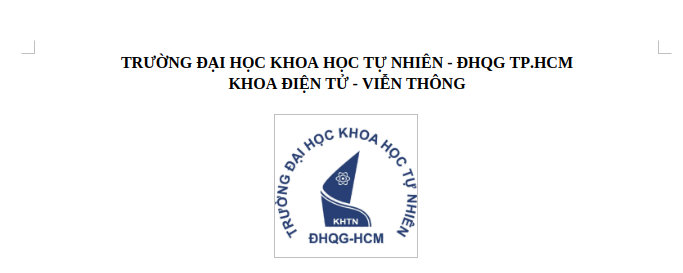
\includegraphics[width=31mm,trim=270 14 270 112,clip]{khtn_reference.png}\par
}{\vspace{31mm}}
\vspace{10mm}
{\Large\bfseries THIẾT KẾ VI MẠCH TƯƠNG TỰ NÂNG CAO\par}
\vspace{8mm}
{\color{navy}\rule{\textwidth}{1.2pt}\par}\vspace{8mm}
{\Huge\bfseries THIẾT KẾ VÀ PHÂN TÍCH MẠCH THAM CHIẾU BANDGAP TOÀN CMOS\par}
\vspace{7mm}
{\Large Công nghệ GPDK090, nguồn nuôi \VDDnom, điện áp tham chiếu \VREFtarget\par}
\vspace{8mm}
{\color{navy}\rule{\textwidth}{1.2pt}\par}
\vfill
\begin{tabular}{rl}
\textbf{Sinh viên:}&Lê Phan Thanh Liêm\\
\textbf{Môi trường thiết kế:}&Cadence Virtuoso / Spectre\\
\textbf{Công nghệ:}&GPDK090 BSIM3\\
\textbf{Thời gian:}&Tháng 11 năm 2026
\end{tabular}
\vfill
\end{titlepage}

\pagenumbering{roman}

% -----------------------------------------------------------------------------
% TÓM TẮT
% -----------------------------------------------------------------------------
\chapter*{Tóm tắt}
\addcontentsline{toc}{chapter}{Tóm tắt}
Báo cáo trình bày quy trình thiết kế và kiểm chứng một mạch tham chiếu bandgap
toàn CMOS dựa trên phương pháp của Madeira và Paulino~\cite{madeira2017}. Hai
transistor NMOS mắc diode được phân cực ở các mức đảo khác nhau để tạo ra các
thành phần dòng có hệ số nhiệt CTAT và PTAT. Một OTA đầu vào PMOS cưỡng bức hai
nút cảm biến gần bằng nhau; các gương dòng PMOS sao chép dòng tổng sang nhánh
ngõ ra để tạo điện áp tham chiếu trên điện trở tải.

Phiên bản đang thiết kế sử dụng nguồn nuôi danh định \VDDnom{} và hướng tới
$V_{REF}=\VREFtarget$ trong dải nhiệt độ \Tmin{} đến \Tmax. OTA sử dụng dòng
phân cực \IBIASota, mạng bù Miller $R_z=\RzFinal$ và $C_C=\CcFinal$. Kết quả
sơ bộ tại điều kiện danh định cho $V_{REF}\approx\SI{599.7}{mV}$, độ biến thiên
toàn dải nhiệt khoảng \SI{8}{mV} và hệ số nhiệt xấp xỉ
\SI{95}{ppm/^{\circ}C}. Các kết quả line regulation, PSRR, startup, PVT,
Monte Carlo và hậu layout sẽ được bổ sung sau khi hoàn tất mô phỏng.

\tableofcontents
\clearpage
\pagenumbering{arabic}

% =============================================================================
\chapter{Giới thiệu và yêu cầu thiết kế}
% =============================================================================

\section{Bối cảnh}
Điện áp tham chiếu là khối cơ bản trong bộ ổn áp LDO, bộ chuyển đổi dữ liệu,
cảm biến và các hệ thống quản lý nguồn. Giá trị tham chiếu cần ít phụ thuộc vào
nhiệt độ, điện áp nguồn và sai lệch công nghệ. Bandgap truyền thống dùng transistor
lưỡng cực để tổng hợp một điện áp CTAT và một điện áp PTAT. Đối với nguồn thấp,
kiến trúc toàn CMOS có thể thay thế transistor lưỡng cực bằng MOS hoạt động trong
vùng đảo yếu, nơi dòng điện phụ thuộc hàm mũ vào $V_{GS}$~\cite{madeira2017}.

\section{Mục tiêu đồ án}
Mục tiêu là thiết kế lại mạch tham chiếu trong bài báo cho công nghệ GPDK090 và
thay đổi điểm làm việc từ cấu hình gốc \SI{0.45}{V} sang điện áp tham chiếu
\VREFtarget{} tại nguồn \VDDnom. Thiết kế phải được kiểm tra ở mức transistor,
không chỉ dựa trên mô hình square-law hoặc giả thiết dòng gương lý tưởng.

\section{Thông số mục tiêu}
\begin{table}[H]
\centering
\caption{Thông số mục tiêu của mạch bandgap.}
\begin{tabularx}{\textwidth}{>{\bfseries}l >{\raggedright\arraybackslash}X l}
\toprule
Thông số & Giá trị mục tiêu / điều kiện & Ký hiệu\\
\midrule
Nguồn nuôi danh định & \VDDnom, $V_{SS}=\SI{0}{V}$ & $V_{DD}$\\
Điện áp tham chiếu & \VREFtarget{} tại \SI{27}{^{\circ}C} & $V_{REF}$\\
Dải nhiệt độ & \Tmin{} đến \Tmax & $T$\\
Hệ số nhiệt & mục tiêu nhỏ hơn \SI{100}{ppm/^{\circ}C} & TC\\
Sai số danh định & \TBD{quy định sai số, ví dụ $\pm1\%$} & $\varepsilon_{VREF}$\\
Nguồn nhỏ nhất & \TBD{giá trị cần xác minh bằng DC sweep} & $V_{DD,min}$\\
Line regulation & \TBD{mV/V hoặc \%/V} & LR\\
PSRR & \TBD{mức mục tiêu và dải tần} & PSRR\\
Công suất tĩnh & \TBD{giới hạn công suất} & $P_{DC}$\\
Startup & tự khởi động ở mọi corner và tốc độ ramp nguồn & $t_{start}$\\
\bottomrule
\end{tabularx}
\end{table}

\section{Đóng góp và phạm vi báo cáo}
Báo cáo tập trung vào thiết kế schematic và kiểm chứng bằng Spectre. Các kết quả
layout, DRC, LVS và PEX được tổ chức thành chương riêng để bổ sung sau. Những giá
trị chưa có hình mô phỏng hoặc chưa được xác minh ở PVT được đánh dấu rõ bằng
\pending.

% =============================================================================
\chapter{Cơ sở lý thuyết của bandgap toàn CMOS}
% =============================================================================

\section{Dòng MOS trong vùng đảo yếu}
Trong vùng đảo yếu và khi transistor đã bão hòa, dòng drain của NMOS có thể
được mô tả gần đúng bởi
\begin{equation}
I_D \simeq I_0\frac{W}{L}
\exp\!\left(\frac{V_{GS}-V_{TH}}{nV_T}\right),
\qquad
V_T=\frac{kT}{q},
\label{eq:subthreshold-current}
\end{equation}
trong đó $I_0$ là dòng đặc trưng công nghệ, $n$ là hệ số slope dưới ngưỡng,
$k$ là hằng số Boltzmann và $q$ là điện tích electron. Quan hệ hàm mũ này cho
phép dùng MOS mắc diode để tạo các điện áp CTAT và PTAT tương tự transistor BJT.

\section{Điện áp CTAT và PTAT}
Điện áp $V_{GS}$ của một NMOS phân cực ở dòng gần cố định giảm khi nhiệt độ
tăng, nên được dùng làm đại lượng CTAT. Với hai transistor có tỷ số hình học
hoặc mật độ dòng khác nhau, hiệu điện áp cổng--nguồn có dạng gần đúng
\begin{equation}
\Delta V_{GS}=V_{GS,5}-V_{GS,8}
\simeq nV_T\ln\!\left(
\frac{I_5/(W/L)_5}{I_8/(W/L)_8}
\right),
\label{eq:delta-vgs}
\end{equation}
và có hệ số nhiệt dương do $V_T=kT/q$ tăng tuyến tính theo nhiệt độ.

\section{Phương trình dòng tham chiếu}
Với gain OTA đủ lớn để hai nút cảm biến gần bằng nhau, áp dụng KCL cho mạng
$R_1$--$R_2$ cho dòng nhánh tham chiếu
\begin{equation}
I_D=\frac{V_{GS,5}-V_{GS,8}}{R_1}
   +\frac{V_{GS,5}}{R_2}.
\label{eq:iref}
\end{equation}
Thành phần thứ nhất chủ yếu PTAT, thành phần thứ hai chủ yếu CTAT. Gương dòng
chép $I_D$ sang nhánh ngõ ra, do đó
\begin{equation}
V_{REF}=R_3 I_D
=R_3\left[
\frac{\Delta V_{GS}}{R_1}+\frac{V_{GS,5}}{R_2}
\right].
\label{eq:vref}
\end{equation}

\section{Điều kiện bù nhiệt bậc một}
Điều kiện first-order để điện áp tham chiếu có độ dốc bằng không tại nhiệt độ
thiết kế $T_0$ là
\begin{equation}
\left.\frac{\dd V_{REF}}{\dd T}\right|_{T=T_0}=0.
\end{equation}
Từ~\eqref{eq:vref}, bỏ qua hệ số nhiệt của điện trở,
\begin{equation}
\frac{1}{R_1}\frac{\dd\Delta V_{GS}}{\dd T}
+\frac{1}{R_2}\frac{\dd V_{GS,5}}{\dd T}=0,
\end{equation}
suy ra tỷ số khởi đầu
\begin{equation}
\boxed{
\frac{R_2}{R_1}
=-\frac{\dd V_{GS,5}/\dd T}
        {\dd\Delta V_{GS}/\dd T}}
\label{eq:r-ratio}
\end{equation}
Tỷ số này chỉ là first-cut. Trong mạch thật, dòng gương bị chia giữa $R_1$ và
$R_2$, điện trở có hệ số nhiệt, $r_o$ hữu hạn và các transistor không hoàn toàn
ở cùng vùng đảo. Vì vậy giá trị cuối phải được tối ưu lại bằng mô phỏng.

\section{Định nghĩa các chỉ tiêu}
Hệ số nhiệt theo phương pháp max--min được dùng trong báo cáo:
\begin{equation}
TC=\frac{V_{REF,max}-V_{REF,min}}
{V_{REF}(T_0)(T_{max}-T_{min})}\times10^6
\quad[\mathrm{ppm}/^{\circ}\mathrm C].
\label{eq:tc}
\end{equation}
Line regulation được tính bởi
\begin{equation}
LR=\frac{\Delta V_{REF}}{\Delta V_{DD}}
\quad[\mathrm{V/V}],
\end{equation}
và PSRR được biểu diễn theo quy ước dương
\begin{equation}
PSRR(f)=20\log_{10}\left|
\frac{v_{dd}(f)}{v_{ref}(f)}
\right|.
\label{eq:psrr}
\end{equation}

% =============================================================================
\chapter{Kiến trúc mạch và phương pháp thiết kế}
% =============================================================================

\section{Kiến trúc tổng thể}
Mạch được phát triển từ kiến trúc đề xuất trong~\cite{madeira2017}. Các khối
chức năng gồm:
\begin{itemize}[leftmargin=16mm]
\item M1--M2 và các nhánh bias: tạo các mức dòng cần thiết cho lõi CMOS;
\item M5 và M8: NMOS mắc diode tạo $V_{GS,5}$ và $V_{GS,8}$;
\item $R_1$ và $R_2$: tổng hợp dòng PTAT và CTAT;
\item M3--M4, M6--M7 và M9: sao chép dòng giữa các nhánh;
\item OTA đầu vào PMOS: cân bằng hai nút cảm biến ở common-mode thấp;
\item $R_3$: chuyển dòng tham chiếu thành $V_{REF}$;
\item $C_{OUT}$: lọc nhiễu và xác lập cực tại ngõ ra.
\end{itemize}

\placeholderfig{67mm}{Sơ đồ nguyên lý đầy đủ của BGR tại $V_{DD}=\SI{1.2}{V}$.}

\section{Phương pháp khảo sát transistor mắc diode}
Hai NMOS mắc diode được mô phỏng độc lập ở dòng mục tiêu. Nhiệt độ được sweep
từ \Tmin{} đến \Tmax{} cho nhiều giá trị $W/L$. Từ các đường $V_{GS}(T)$,
trích:
\begin{itemize}[leftmargin=16mm]
\item $V_{GS}$ tại \SI{27}{^{\circ}C};
\item độ dốc $\dd V_{GS}/\dd T$;
\item $g_m/I_D$ hoặc inversion coefficient để phân loại vùng đảo;
\item độ cong bậc cao theo nhiệt độ.
\end{itemize}

\placeholderfig{60mm}{Testbench khảo sát NMOS mắc diode tại dòng phân cực mục tiêu.}
\placeholderfig{62mm}{Các đường $V_{GS}(T)$ theo kích thước transistor.}

\begin{table}[H]
\centering
\caption{Kết quả khảo sát NMOS mắc diode.}
\small
\resizebox{\textwidth}{!}{%
\begin{tabular}{ccccc}
\toprule
$W$ ($\micro$m)&$L$ ($\micro$m)&$I_D$&$V_{GS}(27^{\circ}C)$&$\dd V_{GS}/\dd T$\\
\midrule
\TBD{M5}&\TBD{M5}&\TBD{dòng}&\TBD{giá trị}&\TBD{mV/$^{\circ}$C}\\
\TBD{M8}&\TBD{M8}&\TBD{dòng}&\TBD{giá trị}&\TBD{mV/$^{\circ}$C}\\
\bottomrule
\end{tabular}}
\end{table}

\section{Tính first-cut cho điện trở}
Từ các độ dốc đo được, dùng~\eqref{eq:r-ratio} để tìm tỷ số ban đầu
$R_2/R_1$. Tổng trở được chọn theo giới hạn công suất và diện tích. Sau đó
$R_3$ được tính từ dòng nhánh danh định:
\begin{equation}
R_3=\frac{V_{REF,target}}{I_{D,nom}}.
\label{eq:r3}
\end{equation}

\begin{table}[H]
\centering
\caption{Giá trị điện trở và tụ của phiên bản schematic hiện tại.}
\begin{tabular}{lll}
\toprule
Phần tử&Giá trị&Vai trò\\
\midrule
$R_1$&\RoneFinal&Đặt độ lớn thành phần PTAT\\
$R_2$&\RtwoFinal&Đặt độ lớn thành phần CTAT\\
$R_3$&\RthreeFinal&Đặt mức $V_{REF}$\\
$C_{OUT}$&\CoutFinal&Lọc ngõ ra / tải BGR\\
\bottomrule
\end{tabular}
\end{table}

\section{Kích thước transistor}
\begin{table}[H]
\centering
\caption{Kích thước transistor của lõi BGR.}
\begin{tabular}{ccccp{55mm}}
\toprule
Nhóm MOS&$W$ ($\micro$m)&$L$ ($\micro$m)&$m$&Chức năng\\
\midrule
M1&0.64&10&1&Nhánh bias bên trái\\
M2&5&10&1&NMOS nhánh bias\\
M3, M6, M9&8&2&1&Gương dòng PMOS\\
M4, M7&3&3&1&Cascade / dịch mức nhánh PMOS\\
M5&5&10&1&NMOS mắc diode thứ nhất\\
M8&20&10&\TBD{m}&NMOS mắc diode thứ hai\\
\bottomrule
\end{tabular}
\end{table}

Các giá trị trên phải được đối chiếu lại với schematic cuối cùng trước khi nộp.
Đặc biệt cần ghi rõ multiplicity của M8 và cách quy đổi sang $W_{eff}$.

% =============================================================================
\chapter{Thiết kế OTA đầu vào PMOS}
% =============================================================================

\section{Yêu cầu đối với OTA trong BGR}
Hai nút cảm biến của lõi BGR nằm ở common-mode thấp, do đó cặp vi sai PMOS phù
hợp hơn cặp NMOS. OTA cần có gain đủ lớn để giảm sai số giữa hai đầu vào, output
swing đủ cao để điều khiển gate gương PMOS và ổn định với tải của vòng BGR.

\placeholderfig{65mm}{Sơ đồ transistor của OTA đầu vào PMOS và mạng bù Miller.}

\section{Kích thước và mạng bù}
\begin{table}[H]
\centering
\caption{Kích thước OTA đầu vào PMOS tại \VDDnom.}
\begin{tabular}{ccccp{54mm}}
\toprule
MOS&$W$ ($\micro$m)&$L$ ($\micro$m)&$m$&Chức năng\\
\midrule
M1, M2&2&10&1&Cặp vi sai PMOS\\
M3, M4&0.5&10&1&Gương tải NMOS\\
M5&3.8&10&1&Nguồn dòng cặp vào\\
M8&1.9&10&1&PMOS mắc diode tạo bias\\
M6&1.2&10&1&Tầng hai NMOS common-source\\
M7&4.6&10&1&Tải dòng PMOS tầng hai\\
\bottomrule
\end{tabular}
\end{table}

Từ operating point của M6, $g_{m6}\approx\SI{4.45}{\micro S}$, do đó điện trở
nulling first-cut là
\begin{equation}
R_z\simeq\frac{1}{g_{m6}}\approx\SI{225}{k\ohm}.
\end{equation}
Giá trị mô phỏng hiện tại là $R_z=\RzFinal$ và $C_C=\CcFinal$.

\section{Kết quả DC và STB sơ bộ}
Ở cấu hình voltage follower, kết quả sơ bộ cho
\begin{align}
A_{loop,0}&\approx\SI{78.83}{dB},\\
f_u&\approx\SI{361.7}{kHz},\\
PM&\approx\ang{60.9}.
\end{align}

\placeholderfig{60mm}{Operating point của OTA ở cấu hình voltage follower.}
\placeholderfig{62mm}{Đáp ứng STB của OTA với $R_z=\RzFinal$ và $C_C=\CcFinal$.}

Kết quả follower chỉ chứng minh OTA độc lập. Khi OTA được đặt trong BGR, tải,
điểm phân cực output và hệ số hồi tiếp thay đổi; do đó phải chạy STB lại cho
toàn vòng BGR.

% =============================================================================
\chapter{Phân tích DC và nhiệt độ}
% =============================================================================

\section{Operating point danh định}
Phép phân tích DC được thực hiện tại $V_{DD}=\VDDnom$, $T=\SI{27}{^{\circ}C}$.
Cần lưu lại điện áp tất cả các nút, dòng từng nhánh, region, $V_{DS}$,
$V_{DSAT}$, $g_m$ và $g_{ds}$ của từng transistor.

\placeholderfig{72mm}{Operating point của toàn mạch BGR tại điều kiện danh định.}

\begin{table}[H]
\centering
\caption{Bảng operating point danh định của lõi BGR.}
\small
\resizebox{\textwidth}{!}{%
\begin{tabular}{cccccc}
\toprule
MOS&$I_D$&$g_m$&$g_{ds}$&$V_{DS}-V_{DSAT}$&Region\\
\midrule
M1&\TBD{ }&\TBD{ }&\TBD{ }&\TBD{ }&\TBD{ }\\
M2&\TBD{ }&\TBD{ }&\TBD{ }&\TBD{ }&\TBD{ }\\
M3--M9&\multicolumn{5}{c}{\TBD{bổ sung từ Results Display Window}}\\
\bottomrule
\end{tabular}}
\end{table}

\section{Điện áp tham chiếu theo nhiệt độ}
Nhiệt độ được sweep từ \Tmin{} đến \Tmax. Các điện trở $R_1$ và $R_2$ được
tinh chỉnh để hai đầu dải nhiệt gần bằng nhau, sau đó $R_3$ được dùng để đưa
$V_{REF}(27^{\circ}C)$ về \VREFtarget.

\placeholderfig{68mm}{$V_{REF}$ theo nhiệt độ sau khi tối ưu $R_1/R_2$.}

Kết quả sơ bộ:
\begin{align}
V_{REF}(27^{\circ}C)&\approx\SI{599.7}{mV},\\
V_{REF,max}-V_{REF,min}&\approx\SI{8.0}{mV},\\
TC&\approx\SI{95}{ppm/^{\circ}C}.
\end{align}

\section{Nhận xét curvature}
\TBD{Giải thích dạng chữ U của đường nhiệt độ, vị trí cực tiểu, giới hạn của
bù bậc một và ảnh hưởng của vùng đảo M5/M8.}

% =============================================================================
\chapter{Line regulation và dải nguồn hoạt động}
% =============================================================================

\section{Thiết lập mô phỏng}
Sweep $V_{DD}$ từ \SI{0}{V} đến \TBD{điện áp cực đại, ví dụ \SI{1.5}{V}} tại
\SI{27}{^{\circ}C}. Quan sát đồng thời $V_{REF}$, output OTA, hai đầu vào OTA
và dòng M9.

\placeholderfig{65mm}{Testbench và thiết lập DC sweep theo $V_{DD}$.}
\placeholderfig{65mm}{$V_{REF}$ theo $V_{DD}$ và xác định $V_{DD,min}$.}

\section{Kết quả}
\begin{table}[H]
\centering
\caption{Kết quả line regulation.}
\begin{tabular}{ll}
\toprule
Đại lượng&Giá trị\\
\midrule
$V_{DD,min}$&\TBD{V}\\
$V_{REF}$ tại $V_{DD}=\SI{1.0}{V}$&\TBD{mV}\\
$V_{REF}$ tại $V_{DD}=\SI{1.2}{V}$&\TBD{mV}\\
$V_{REF}$ tại $V_{DD}=\SI{1.4}{V}$&\TBD{mV}\\
Line regulation&\TBD{mV/V}\\
\bottomrule
\end{tabular}
\end{table}

\TBD{Nhận xét cơ chế mất regulation ở nguồn thấp và transistor giới hạn
headroom.}

% =============================================================================
\chapter{Ổn định vòng lặp và đáp ứng khởi động}
% =============================================================================

\section{Phân tích STB của vòng BGR}
Một iprobe được đặt nối tiếp trong đường từ output OTA đến bus điều khiển gương
PMOS. Phép STB được thực hiện tại điều kiện danh định và lặp lại ở các corner
quan trọng.

\placeholderfig{62mm}{Vị trí iprobe trong vòng hồi tiếp của BGR.}
\placeholderfig{65mm}{Loop gain và phase của vòng BGR.}

\begin{table}[H]
\centering
\caption{Các chỉ tiêu ổn định của vòng BGR.}
\begin{tabular}{llc}
\toprule
Thông số&Kết quả&Đánh giá\\
\midrule
DC loop gain&\TBD{dB}&\pending\\
Unity-gain frequency&\TBD{Hz}&\pending\\
Phase margin&\TBD{độ}&\pending\\
Gain margin&\TBD{dB}&\pending\\
\bottomrule
\end{tabular}
\end{table}

\section{Startup transient}
Nguồn VDD được ramp từ 0 đến \VDDnom{} với các rise time khác nhau. Mạch phải
thoát khỏi nghiệm dòng bằng không và hội tụ về \VREFtarget{} mà không dao động
kéo dài.

\begin{table}[H]
\centering
\caption{Các điều kiện startup cần kiểm tra.}
\begin{tabular}{ccc}
\toprule
Rise time nguồn&Thời gian mô phỏng&Kết quả\\
\midrule
\SI{1}{\micro s}&\SI{5}{ms}&\TBD{ }\\
\SI{100}{\micro s}&\SI{5}{ms}&\TBD{ }\\
\SI{1}{ms}&\SI{10}{ms}&\TBD{ }\\
\SI{10}{ms}&\SI{40}{ms}&\TBD{ }\\
\bottomrule
\end{tabular}
\end{table}

\placeholderfig{65mm}{Đáp ứng startup của $V_{DD}$, $V_{REF}$, output OTA và hai nút cảm biến.}

\section{Settling và overshoot}
\TBD{Định nghĩa dải $\pm1\%$, đo settling time sau khi VDD đạt giá trị cuối,
đo overshoot VREF và thảo luận ảnh hưởng tới LDO.}

% =============================================================================
\chapter{PSRR và nhiễu}
% =============================================================================

\section{Thiết lập PSRR}
Nguồn VDD có giá trị DC \VDDnom{} và biên độ AC bằng \SI{1}{V}. Khi đó hàm
truyền nguồn--ngõ ra là $v_{ref}/v_{dd}=v_{ref}$. Theo quy ước dương trong
\eqref{eq:psrr}, biểu thức Calculator có thể dùng là
\begin{equation}
-20\log_{10}|V_{REF}(f)|.
\end{equation}

\placeholderfig{60mm}{Testbench AC dùng để đo PSRR.}
\placeholderfig{65mm}{PSRR của BGR theo tần số.}

\section{Ảnh hưởng của tụ ngõ ra}
Sweep $C_{OUT}$ để phân biệt ảnh hưởng của cực ngõ ra với đường feedthrough qua
OTA và gương PMOS. Mỗi giá trị tụ phải được đánh giá đồng thời bằng PSRR và STB.

\begin{table}[H]
\centering
\caption{PSRR tại các tần số đại diện.}
\small
\resizebox{\textwidth}{!}{%
\begin{tabular}{ccccc}
\toprule
$C_{OUT}$&\SI{1}{Hz}&\SI{1}{kHz}&\SI{10}{kHz}&\SI{1}{MHz}\\
\midrule
\TBD{pF}&\TBD{dB}&\TBD{dB}&\TBD{dB}&\TBD{dB}\\
\bottomrule
\end{tabular}}
\end{table}

\section{Noise}
\TBD{Bổ sung output-referred noise, integrated noise trong dải tần quan tâm và
đóng góp của OTA, điện trở, transistor mắc diode.}

% =============================================================================
\chapter{PVT, mismatch và Monte Carlo}
% =============================================================================

\section{Process corners}
Các corner NN, FF, SS, FS và SF được chạy riêng. Tại mỗi corner, kiểm tra nhiệt
độ, nguồn, operating point và startup. Không gộp nhiều model section vào cùng
một lần netlist.

\begin{table}[H]
\centering
\caption{Ma trận PVT tối thiểu.}
\small
\resizebox{\textwidth}{!}{%
\begin{tabular}{cccccc}
\toprule
Corner&$V_{DD}$&Nhiệt độ&$V_{REF}$&TC&Startup\\
\midrule
NN&\SI{1.2}{V}&\SI{27}{^{\circ}C}&\TBD{ }&\TBD{ }&\TBD{ }\\
SS&\TBD{min}&\Tmin&\TBD{ }&\TBD{ }&\TBD{ }\\
FF&\TBD{max}&\Tmax&\TBD{ }&\TBD{ }&\TBD{ }\\
FS/SF&\TBD{ }&\TBD{ }&\TBD{ }&\TBD{ }&\TBD{ }\\
\bottomrule
\end{tabular}}
\end{table}

\section{Monte Carlo}
\TBD{Thiết lập số lần chạy, tách process và mismatch, thống kê mean, sigma,
min/max của VREF và TC.}

\placeholderfig{62mm}{Histogram Monte Carlo của $V_{REF}(27^{\circ}C)$.}

\section{Trim}
Nếu sai số mismatch vượt specification, mạng trim có thể được bố trí trên
$R_3$ để hiệu chỉnh mức điện áp và trên tỷ số $R_1/R_2$ để hiệu chỉnh độ dốc
nhiệt. \TBD{Bổ sung số bit trim và bước LSB nếu triển khai.}

% =============================================================================
\chapter{Layout vật lý}
% =============================================================================

\section{Nguyên tắc matching}
Các transistor trong cùng gương dòng phải cùng hướng, cùng môi trường và được
đặt đối xứng. Các phần tử cần matching tốt nên dùng common-centroid,
interdigitation và dummy. Điện trở $R_1$, $R_2$, $R_3$ cần cùng loại vật liệu
và được chia segment để kiểm soát gradient.

\section{Định tuyến và cách ly}
Các nút trở kháng cao của OTA và bus gate gương PMOS phải ngắn, tránh ghép với
VDD và VREF. Guard ring, substrate contact và decoupling được bố trí để giảm
nhiễu nền và latch-up.

\placeholderfig{67mm}{Layout toàn mạch BGR.}
\placeholderfig{67mm}{Extracted view và các parasitic chính.}

\section{DRC, LVS và PEX}
\begin{table}[H]
\centering
\caption{Tình trạng kiểm tra vật lý.}
\begin{tabular}{lll}
\toprule
Kiểm tra&Kết quả&Ghi chú\\
\midrule
DRC&\TBD{ }&\TBD{ }\\
LVS&\TBD{ }&\TBD{ }\\
PEX&\TBD{ }&\TBD{ }\\
\bottomrule
\end{tabular}
\end{table}

% =============================================================================
\chapter{Kết quả và thảo luận}
% =============================================================================

\section{Tổng hợp thông số}
\begin{table}[H]
\centering
\caption{Tổng hợp specification và kết quả mô phỏng.}
\begin{tabularx}{\textwidth}{>{\bfseries}l l l >{\raggedright\arraybackslash}X}
\toprule
Chỉ tiêu&Mục tiêu&Kết quả&Đánh giá\\
\midrule
$V_{REF}(27^{\circ}C)$&\SI{600}{mV}&\measured{\SI{599.7}{mV}}&\pass\\
Temperature coefficient&$<\SI{100}{ppm/^{\circ}C}$&\measured{$\approx\SI{95}{ppm/^{\circ}C}$}&\pass\\
Biến thiên \Tmin{}--\Tmax&\TBD{mV}&\measured{$\approx\SI{8}{mV}$}&\pending\\
$V_{DD,min}$&\TBD{V}&\TBD{V}&\pending\\
Line regulation&\TBD{mV/V}&\TBD{mV/V}&\pending\\
PSRR&\TBD{dB}&\TBD{dB}&\pending\\
Phase margin BGR&$\ge\ang{60}$&\TBD{độ}&\pending\\
Startup&mọi điều kiện PVT&\TBD{ }&\pending\\
Công suất&\TBD{$\micro$W}&\TBD{$\micro$W}&\pending\\
Monte Carlo&\TBD{yield}&\TBD{ }&\pending\\
\bottomrule
\end{tabularx}
\end{table}

\section{Đánh đổi chính}
\begin{itemize}[leftmargin=16mm]
\item Tăng điện trở làm giảm công suất nhưng tăng diện tích, nhiễu nhiệt và độ
nhạy với dòng rò.
\item Tăng chiều dài kênh cải thiện $r_o$ và matching nhưng tăng diện tích và
điện dung ký sinh.
\item Tăng $C_{OUT}$ cải thiện lọc cao tần nhưng làm startup chậm và có thể thay
đổi pole của vòng hồi tiếp.
\item OTA gain cao giảm sai số cân bằng nút nhưng cần được bù ổn định trong
toàn vòng BGR, không chỉ trong follower.
\item Bù nhiệt bậc một không loại bỏ curvature bậc cao của $V_{GS}(T)$.
\end{itemize}

\section{So sánh với bài báo tham khảo}
\begin{table}[H]
\centering
\caption{So sánh sơ bộ với thiết kế của Madeira và Paulino.}
\begin{tabular}{lll}
\toprule
Thông số&Bài báo~\cite{madeira2017}&Thiết kế này\\
\midrule
Công nghệ&\SI{130}{nm}&GPDK090\\
$V_{REF}$&\SI{0.45}{V}&\SI{0.60}{V}\\
$V_{DD,min}$&\SI{0.6}{V}&\TBD{V}\\
Dải nhiệt&\SIrange{-40}{100}{^{\circ}C}&\SIrange{-40}{100}{^{\circ}C}\\
Biến thiên nhiệt&\SI{1.54}{mV}&\measured{$\approx\SI{8}{mV}$}\\
TC&\SI{24}{ppm/^{\circ}C}&\measured{$\approx\SI{95}{ppm/^{\circ}C}$}\\
PSRR&khoảng \SI{40}{dB} dưới \SI{20}{kHz}&\TBD{dB}\\
\bottomrule
\end{tabular}
\end{table}

% =============================================================================
\chapter{Kết luận}
% =============================================================================

Báo cáo đã xây dựng khung thiết kế cho một BGR toàn CMOS ở \VDDnom{} với điện
áp tham chiếu mục tiêu \VREFtarget. Kết quả nominal ban đầu cho thấy mức điện
áp và hệ số nhiệt đã đạt mục tiêu sơ bộ. Tuy nhiên, kết luận cuối cùng chỉ được
đưa ra sau khi hoàn tất line regulation, STB toàn vòng, PSRR, startup, PVT,
Monte Carlo và mô phỏng hậu layout.

\TBD{Viết lại kết luận sau khi hoàn tất toàn bộ hình và bảng kết quả.}

% =============================================================================
\appendix
\chapter{Định nghĩa phép đo trong Cadence}
% =============================================================================

\section{Temperature coefficient}
\begin{equation}
TC=\frac{\max(V_{REF})-\min(V_{REF})}
{V_{REF}(27^{\circ}C)(T_{max}-T_{min})}\times10^6.
\end{equation}

\section{PSRR}
Nếu nguồn VDD có AC magnitude bằng \SI{1}{V}, biểu thức Calculator theo quy
ước PSRR dương là
\begin{verbatim}
-dB20(VF("/VREF"))
\end{verbatim}
Cần chọn đúng result ``ac''; nếu VF trả về nil thì ADE đang trỏ tới result STB
hoặc transient.

\section{STB}
Chèn iprobe nối tiếp trong vòng cần khảo sát, chọn instance đó trong analysis
STB và đọc loop gain, unity frequency, phase margin, gain margin. Điểm đo phải
giữ nguyên bias DC của mạch.

\chapter{Danh sách hình cần bổ sung}
\begin{enumerate}
\item Schematic BGR hoàn chỉnh và operating point danh định.
\item Testbench NMOS mắc diode và $V_{GS}(T)$.
\item Schematic OTA PMOS, operating point và STB follower.
\item $V_{REF}(T)$ trước và sau khi tối ưu $R_1/R_2$.
\item $V_{REF}(V_{DD})$ và xác định $V_{DD,min}$.
\item STB của toàn vòng BGR.
\item Startup với nhiều rise time nguồn.
\item PSRR theo tần số và sweep $C_{OUT}$.
\item PVT, Monte Carlo và histogram.
\item Layout, DRC, LVS và extracted view.
\end{enumerate}

% =============================================================================
% TÀI LIỆU THAM KHẢO
% =============================================================================
\begin{thebibliography}{9}

\bibitem{madeira2017}
R. Madeira and N. Paulino,
``Design Methodology for an All CMOS Bandgap Voltage Reference Circuit,''
in \emph{Technological Innovation for Smart Systems}, DoCEIS 2017,
pp. 439--446, 2017. DOI: 10.1007/978-3-319-56077-9\_43.

\bibitem{razavi2016}
B. Razavi,
``The Bandgap Reference [A Circuit for All Seasons],''
\emph{IEEE Solid-State Circuits Magazine}, vol. 8, pp. 9--12, 2016.

\bibitem{banba1999}
H. Banba et al.,
``A CMOS bandgap reference circuit with sub-1-V operation,''
\emph{IEEE Journal of Solid-State Circuits}, vol. 34, no. 5,
pp. 670--674, 1999.

\bibitem{yetterdal2003}
T. Ytterdal,
``CMOS bandgap voltage reference circuit for supply voltages down to 0.6 V,''
\emph{Electronics Letters}, vol. 39, pp. 1427--1428, 2003.

\end{thebibliography}

\end{document}
